\section{Fleetio}
%This is what was formerly named Application
This this section is going to focus upon the \textit{Fleetio} solution, this is done since more information is available for \textit{Fleetio} than any of the other solutions.
In order for \textit{Fleetio} to gather data, a mobile application has to be installed on each driver's smart phone.
Initially, static vehicle data has to be manually submitted to the system, however \textit{Fleetio} support the import of vehicle details via the vehicle identification number also know, as VIN, this feature can save some time.

\begin{figure}[h!]
    \centering
    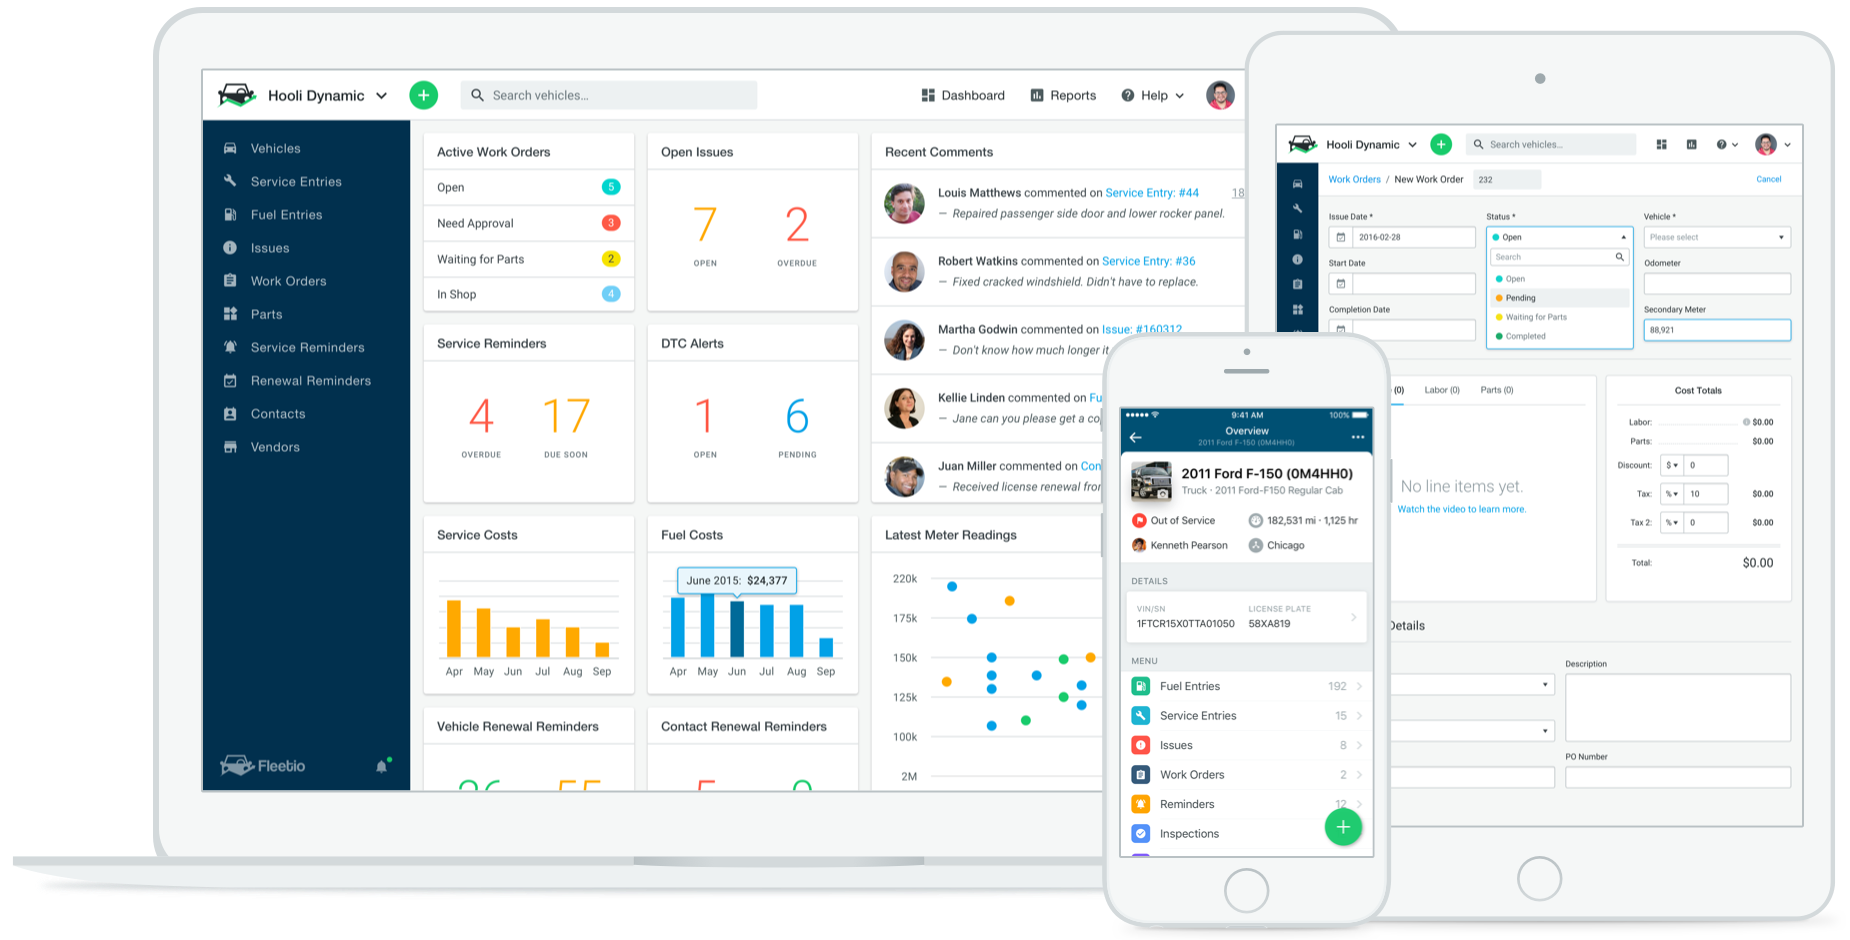
\includegraphics[width=0.5\textwidth]{img/fleetio.png}
    \caption{Display of the Fleetio mobile applications, and Fleetio Dashboard.}
    \label{fig:Fleetio_Devices}
\end{figure}

\subsubsection{Features}\label{ssub:features}
Some of the tools that \textit{Fleetio} support are the following:
\begin{description}
    \item[Vehicle Management] \hfill
    \begin{description}
        \item[Vehicle Profiles] \hfill \\
        Through \textit{Fleetio}, a company is able to create vehicle profiles either manually or through import via VIN. This vehicle information can range from documents to images of the vehicles.
        It is then possible to search through the vehicles which are still in use, and disposed vehicles.
    \end{description}

    \item[Fleet Maintenance] \hfill
    \begin{description}
        \item[Scheduling] \hfill \\
        After all the information has been manually entered into \textit{Fleetio}, a company can then schedule a lot of different vehicle related tasks through the dashboard.
        These things can range from service reminders to preventative maintenance.
        \item[Issue Reporting] \hfill \\
        If a driver spots a problem or experiences any issue with a designated vehicle, the driver can then manually report those issues through the \textit{Fleetio} dashboard.
        After the report has been created an alert is send to the company to inform them of the issue.
        \item[Vendor Overview] \hfill \\
        \textit{Fleetio} makes it possible to map each expense to the different vehicle to the different vendors a company uses.
        \item[Maintenance History] \hfill \\
        Through the \textit{Fleetio} dashboard it is possible to keep track of all the repairs which have been performed on each of the vehicles through the maintenance history, this information must be manually plotted into the system after a repair is done.
    \end{description}

    \item[Driver Management] \hfill
    \begin{description}
        \item[Driver scheduling] \hfill \\
        \textit{Fleetio} supports manual scheduling of each driver and inspections of each vehicle.
        \item[Employee profiles] \hfill \\
        \textit{Fleetio} allows for a company to store information on each of the drivers and its other employees.
        \item[Real--time cost per kilometre] \hfill \\
        \textit{Fleetio} cooperates with multiple different fuel card partners.
        This makes it possible to calculate the cost per kilometre by combining the data from the fuel card partners and the tracking data from \textit{Fleetio}.
        If a fuel card from a non--cooperating company or an alternative payment method has been used, \textit{Fleetio} is still able to calculate the price, however this require the fuelling cost to be manually entered.
     \end{description}
\end{description}
